There are eight sections and subfiles.
Each subfile is empty just after it is generated by newtex.
Editing subfiles is the main work and you need to allocate most of your time to this work.

The first section and subfile are `Installation' and installation.tex respectively.
Maybe you edit a part of the section and test-compile to see how it looks like in the pdf file.
Usually we come and go between editing and test-compiling repeatedly.

If the document is not so big, using rake is the best to test-compile, because it doesn't take much time and the pdf shows the whole document.
This tutorial is rather a small document, so using rake for test-compiling is fine.

\begin{verbatim}
\subsection{Prerequisite}
Buildtools requires the following items.
\begin{enumerate}
\item Linux OS and bash
\item LaTeX system
\item Make or Rake
\end{enumerate}
 ... ...
 ... ...
\end{verbatim}

Then, type the following line to see the pdf.
\begin{verbatim}
$ rake
$ evince Tutorial.pdf
\end{verbatim}

\begin{center}
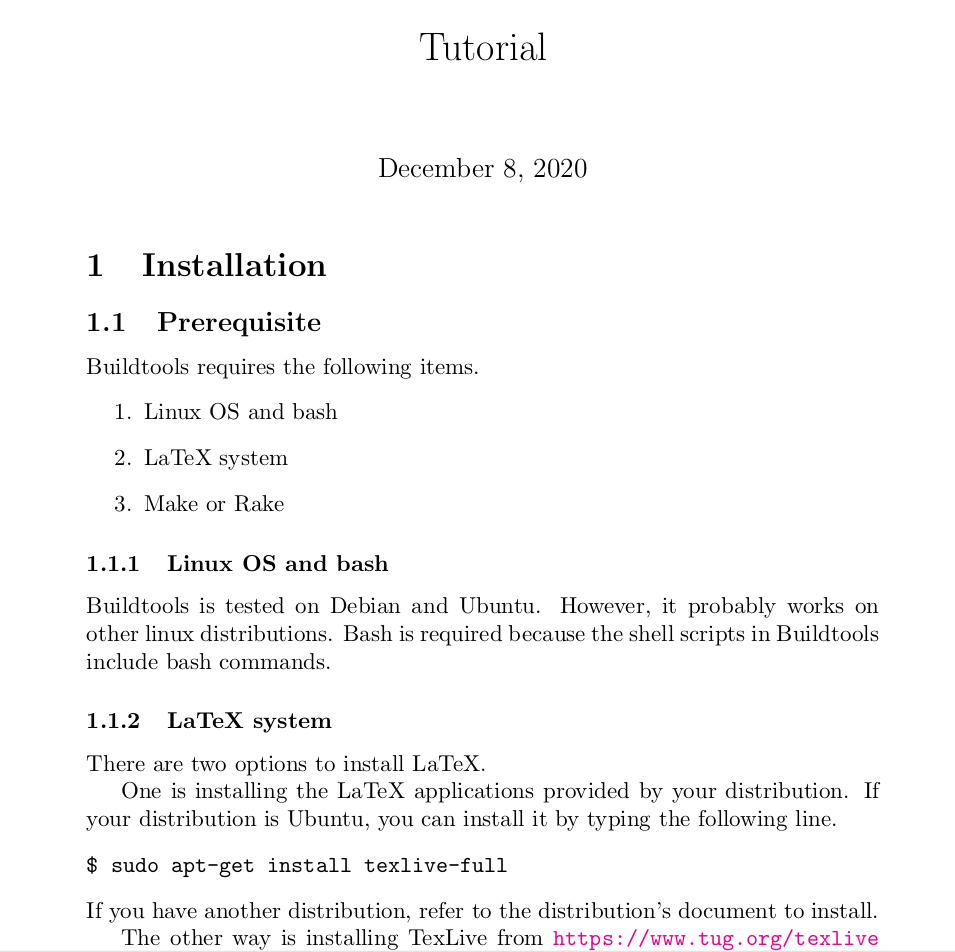
\includegraphics[width=8cm]{Tutorial_2.png}
\end{center}
